\newcommand{\figpath}{Figures}
\newcommand{\totalRows}{6547}
\newcommand{\totalJavaRows}{4239}
\newcommand{\totalJavaScriptRows}{2308}
\newcommand{\totalDiscardedRows}{2985}
\newcommand{\javaDiscardedRows}{2126}
\newcommand{\jsDiscardedRows}{859}
\newcommand{\totalDeletedFiles}{432}
\newcommand{\remainingJavaFileCount}{2113}
\newcommand{\remainingJsFileCount}{1449}
\newenvironment{code}{\captionsetup{type=listing}}{}
\SetupFloatingEnvironment{listing}{name=Source Code}

\chapter{Solution Design and Implementation}\label{sec:design-and-impl-parent}
\section{Solution Design}\label{sec:design}
%%%%%%%%%%%%%%%%%%%%%%%%%%%%%%%%%%%%%%%%%%%%%%%%%%%%%%%%%%%%%%%%%%%%%%%%%%%%%%%%%%%%%%%%%%%%%%%%%%%%%%%%%%%
\subsection{Data Gathered}\label{sec:data-available}
The data collected contained \totalRows{} initially collected in 67 columns. Each record corresponds to a source code file at a given point in time and subsection \ref{sec:data-available} depicts attributes definition through Tables \ref{tbl:available-data-non-repeating-types} to \ref{tbl:available-data-above-0-max-100}, specifying uncommon datatypes found, as well as lists where each attribute in the list has the same properties with regards to data category, data type, and minimum and maximum values present. 

\begin{table}[h!]
\caption{Data Available - non repeating data types}
\label{tbl:available-data-non-repeating-types}
\begin{tabular}{@{}ll@{}}
\toprule
Metric name & Description \\ \midrule
issue key & text \\ 
file path & text \\
source repo & text \\
author & discrete, enumeration of possible authors \\
prev author & discrete, enumeration of possible authors\\
timestamp & continuous, epoch time \\
prev timestamp & continuous, epoch time \\
is bug & boolean, True or False \\
files & ordinal, integer, $\geq{}1$ \\
sqale debt & ratio, integer, $\geq{}0$ \\
statements & ordinal, integer, $\geq{}1$ \\
violations & ratio, integer, $\geq{}0$ \\ \bottomrule
\end{tabular}
\end{table}

\begin{table}[h!]
\caption{Ordinal data, integer, min $\geq{}0 \leq{}100$}
\label{tbl:available-data-above-0-max-100}
\begin{tabular}{@{}l@{}}
\toprule
Metric Name \\ \midrule
branch coverage \\
overall branch coverage \\
overall coverage \\
overall line coverage \\
overall uncovered conditions \\
overall uncovered lines \\ \bottomrule
\end{tabular}
\end{table}


\begin{table}[h!]
\caption{Numeric data, integer, min $\geq{}0$, no definitive maximum}
\label{tbl:available-data-above-0-no-max}
\begin{tabular}{@{}ll@{}}
\toprule
Metric Name & Metric Name \\ \midrule
blocker violations & line coverage \\
bugs & lines \\
classes & lines to cover \\
code smells & major violations \\
comment lines & minor violations \\
comment lines density & ncloc \\
complexity & open issues \\
confirmed issues & public documented API density \\
coverage & public undocumented API \\
critical violations & reliability rating \\
duplicated blocks & reliability remediation effort \\
duplicated files & reopened issues \\
duplicated lines & security rating \\
duplicated lines density & security remediation effort \\
effort to reach maintainability rating A & skipped tests \\
false positive issues & SQALE index \\
file complexity & SQALE rating \\
function complexity & test errors \\
functions & test failures \\
generated lines & test success density \\
generated ncloc & uncovered conditions \\
info violations & uncovered lines \\
it coverage & vulnerabilities \\
it line coverage & wont fix issues \\
it uncovered lines &  \\ \bottomrule
\end{tabular}
\end{table}


\subsection{Data Gathering Components}
The dataset for the analysis had to be generated from live business data as such data has not been made available in the public domain. Section \ref{sec:data-available} can be used a reference as to what metrics, along with their type and brief description, have been gathered. In order to construc the dataset subsequently used in the analysis, 3 real live business tools were used:

\begin{enumerate}{\label{lst:tools_used}}
    \item Sonar server by SonarSource - provided code quality metrics
    \item JIRA by Atlassian  - provided information about file commits as well as the classification of commits into "a bug" or "not a bug" categories
    \item Bitbucket by Atlassian  - provided information about commit timestamp, the author as well as details about previous commit author and previous commit timestamp allowing for calculating file staleness 
\end{enumerate}
    
Additionally, a tool to gather metrics, referred to as Data Gatherer, has been developed in order to produce the end dataset and will be made available upon submission. The purpose of the Data Gatherer tool is to coordinate the execution of other tools from the above list as well as collate the acquired data into the end dataset then used in further analysis as per Figure \ref{fig:data_gathering}.

\begin{figure}[h!]
\centering
    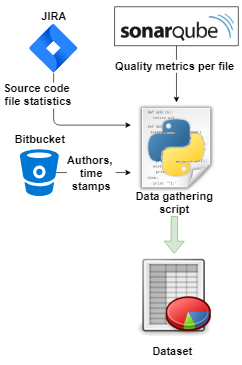
\includegraphics{\figpath/data_arch_small.png}
    \caption{Dataset Gathering operations}
    \label{fig:data_gathering}
\end{figure}

First tool to be used in the data gathering process is Atlassian's JIRA server. JIRA is a ticketing system used by software developers to keep track of issues, feature requests and most importantly in the current context, bugs. Each ticket has been assigned a category upon its creation depicting its purpose. In the context of the current use case the most relevant types encountered are:

\begin{itemize}
    \item Story - represents a feature task to be done. Upon completion it is a fully functional, testable vertical slice of functionality delivering value to end-users
    \item Task - represents an additional development task, such as, but not limited to, setting up test environments, automatization of effort, including testing effort, infrastructure maintenance etc. Does not provide direct value to end users
    \item Bug - represents issues found in released software, especially when expected and actual behaviour of a given piece of functionality doesn't match.
\end{itemize}
Given that Task type tickets are not directly linked to the development life cycle they have been excluded from further analysis and the focus has been placed on Story and Bug type tickets instead.

The second use of JIRA server was its proprietary integration with the source code repository - Bitbucket, as both tools are offered by the same company, Atlassian. For each of the JIRA tickets there existed a link between a given ticket and source code file changes, or commits, made and persisted in Bitbucket system. 
Each commit could consist of many files and each source code file could have been committed to multiple times under the umbrella of a single ticket. However, not all commit records under a ticket have been taken into the account - every so called merge commit have been excluded.

To illustrate what a merge commit is and why it must be excluded \ref{fig:git-branching-merging-and-rebasing} will be used, where blue nodes signify the master, or the golden copy of the code, and green and purple identify branches, where feature, bug fix or any other development work is carried out as part of a development lifecycle. At the end of its life a branch will be integrated into the Master branch, which will generate a merge commit - illustrated by Feature 1 branch. Additionally, it is a normal occurrence to have more than 1 branch created in a given codebase at any given time. If another branch has been created from the master before Feature 1 code was merged, as per \ref{fig:git-branching-merging-and-rebasing} Feature 2, and it is actively being developed on past the merge point such branch will have to be rebased. The rebase process will pull in the merge commit created by Feature 1, however, all source code files listed under merge commit will have already been analyzed under JIRA ticket representing Feature 1, therefore should it not be excluded from further analysis it would have duplicated the effort. Not excluding merge commits also represented significant risk with regards to story vs. bug categorization of source code files committed as Feature 2 might as well have been a bug. In such scenario file committed under Feature 1 ticked would be categorized as non-bug, as per ticket category, as well as bug as per category assigned by the second ticket.

\todo{Need to change Feature 2 to Bug, to illustrate merge commit exclusion better}
\begin{figure}[!h]
    \centering
    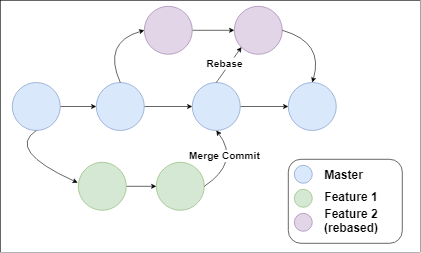
\includegraphics{\figpath/git_branching.png}
    \caption{GIT branching and rebasing strategy}
    \label{fig:git-branching-merging-and-rebasing}
\end{figure}

JIRA ticketing system provided the following columns:
\begin{itemize}
    \item issue key
    \item source repository
    \item file path
    \item category of the record, bug or not a bug
\end{itemize}

while the Bitbucket server provided additional information about:
\begin{itemize}
    \item author
    \item previous author
    \item commit timestamp
    \item timestamp of the previous commit
\end{itemize}

The final tool utilized was SonarQube by SonarSource, an open-source platform. Its capabilities include continuous inspection of code quality to perform automatic reviews with static analysis of code to detect code smells, reports on duplicated code, coding standards, unit tests, code coverage, code complexity, comments,  security vulnerabilities, and much more. In the context of this use case it was utilized to associate code metrics listed in Tables \ref{tbl:available-data-above-0-max-100} and \ref{tbl:available-data-above-0-no-max} as well as \texttt{files}, \texttt{sqale debt}, \texttt{statements} and \texttt{violations} provided in Table \ref{tbl:available-data-non-repeating-types}.

The \texttt{issue key}, \texttt{source repository} and \texttt{file path} were only used to verify that a given data point can be traced to a relevant JIRA ticket in order to verify it belongs to a assigned category, \texttt{author} and \texttt{previous author} were used to populate seniority and project tenure features, \texttt{timestamp} and \texttt{previous timestamp} were used to calculate staleness of the file between changes.



\subsection{Data Modelling}

Once a dataset has been generated as per section \ref{sec:design} it underwent the following operations:
\begin{enumerate}
    \item missing data analysis and data cleaning \label{lst:dataset-ops.item:data-cleaning}
    \item balance of bug to non-bug records in the dataset \label{lst:dataset-ops.item:bug-to-non-bug-balance}
    \item outlier analysis \label{lst:dataset-ops.item:outliers}
    \item data correlation analysis \label{lst:dataset-ops.item:data-correlation}
    \item feature transformation \label{lst:dataset-ops.item:feature-transformation}
    \item feature scaling \label{lst:dataset-ops.item:data-scaling}
    \item relevant feature selection \label{lst:dataset-ops.item:feature-selection}
    \item distribution of selected features \label{lst:dataset-ops.item:attribute-distribution}
    \item evaluation of regularized Logistic Regression model \label{lst:dataset-ops.item:ml-logistic-regression}
    \item evaluation of Decision Tree Classification model \label{lst:dataset-ops.item:ml-decision-tree}
    \item evaluation of additional models as necessary \label{lst:dataset-ops.item:ml-models-additional}
\end{enumerate}

Item \ref{lst:dataset-ops.item:data-cleaning} focuses on cleaning and imputing values for missing metrics. Item \ref{lst:dataset-ops.item:bug-to-non-bug-balance} will focus on listing the ratios between bug and non bug records in the dataset.
Item \ref{lst:dataset-ops.item:outliers} identifies if there are any projects or individual files that are diverging significantly from the rest of the dataset. 
Item \ref{lst:dataset-ops.item:data-correlation} focuses on identifying any feature correlation patterns in order to proceed with feature selection - item  \ref{lst:dataset-ops.item:feature-selection} after which it will be necessary to check for the balance and distribution of the selected features or attributes - which will be the focus of item \ref{lst:dataset-ops.item:attribute-distribution}. Feature distribution is included as part of the analysis as Logistic Regression model is susceptible to non-normally distributed datasets.
Item \ref{lst:dataset-ops.item:data-scaling} concentrates on evaluating multiple scaling methods with regards to their effectiveness of bringing the dataset values to the same scale of magnitude. The scaling method taken into the account are:
\begin{enumerate}
    \item Transformation using natural logarithm - $log(e)$ 
    \item Min-Max scaling
    \item Max-Abs scaling
    \item Standard scaling
    \item Power Transformation using Yeo-Johnson variant
    \item Quantile Transformation using uniform distribution variant
    \item Quantile Transformation using normal distribution variant
\end{enumerate}

\todo{Probably need to talk a bit about what each scaler does and how it works. However, maybe it's better served in the implementation section}
Finally, an evaluation of the effectiveness of selected machine learning models with regards to predicting bug vs non-bug classes in the dataset will be carried out and constitutes the focus of items \ref{lst:dataset-ops.item:ml-logistic-regression}, \ref{lst:dataset-ops.item:ml-decision-tree} and \ref{lst:dataset-ops.item:ml-models-additional} respectively.

\section{Implementation}\label{sec:implementation}
\begin{landscape}

\begin{code}

\captionof{listing}{Main data gathering component - the coordinator}
\label{code:c-code}
\begin{minted}[breaklines]{python}

import sys
import time

import urllib3

from src.author_detail_transformer import AuthorDetailsTransformer
from src.bitbucket import Bitbucket
from src.jira_connector import JiraConnector
from src.sonar_metrics_gatherer import SonarMetricsGatherer


class Gatherer:

    def __init__(self):
        self.header_printed = False

    def main(self, username, password, jira_keys, is_bug_file):
        for jira_key in jira_keys:
            jira_obj = JiraConnector(username, password)
            files, commit_details = jira_obj.main(jira_key)

            sonar_obj = SonarMetricsGatherer(username, password)
            output = []
            bb = Bitbucket(username, password)
            prev_commit_details = bb.get_prev_commit_details_per_filepath(commit_details)
            prev_commit_details = AuthorDetailsTransformer().transform_names_into_codenames(prev_commit_details)

            for file in files.keys():
                repo_file_is_in = files[file]
                component_key = sonar_obj.get_project_key_by_project_name(repo_file_is_in)
                if len(component_key) > 0:
                    # get component_key
                    component_name = sonar_obj.sonar_component_name_generator(component_key, file)
                    if len(component_name) > 0:
                        sorted_metrics_dict = sonar_obj.main(component_name, repo_file_is_in)
                        if len(sorted_metrics_dict) > 0:
                            sorted_metrics_dict['source_repo'] = repo_file_is_in
                            sorted_metrics_dict['is_bug'] = is_bug_file
                            sorted_metrics_dict['issue_key'] = jira_key
                            combined = sorted_metrics_dict.copy()
                            combined.update(prev_commit_details[file])
                            output.append(combined)

                            sonar_obj.save_to_csv(header_printed=self.header_printed, list_of_metric_dicts=output,
                                                  out_path='results.csv')
                            self.header_printed = True
                        else:
                            print('Error with processing JIRA: {0}'.format(jira_key))
                    else:
                        print('Error with processing JIRA: {0}'.format(jira_key))
                else:
                    print('Error with processing JIRA: {0}'.format(jira_key))

    def load_jira_key_files(self, file_location):
        values = []
        with open(file_location) as f:
            for line in f:
                line = line.replace('\n', '')
                values.append(line)
        return values


if __name__ == '__main__':
    start_time = time.time()
    urllib3.disable_warnings()
    password = None
    if len(sys.argv) > 1:
        password = sys.argv[1]
    try:
        obj = Gatherer()
        # get data from bug tickets
        jira_keys = obj.load_jira_key_files('src/resources/tvnx_bug_issue_key_list.dat')
        obj.main('username', password, jira_keys, True)

        # get data from regular tickets
        jira_keys = obj.load_jira_key_files('src/resources/tvnx_story_issue_key_list.dat')
        obj.main('username', password, jira_keys, False)
        print('Operation duration: {0}'.format(time.time() - start_time))
    except Exception as e:
        print('Operation completed with an error. Duration: {0}'.format(time.time() - start_time))

\end{minted}
\end{code}
\end{landscape}